This chapter delves into the development of five prototypes, each portraying a different type of behavior for hands in VR. These different prototypes approach the problem of realism vs sense of embodiment in different ways and to different degrees. The implemented grabbing system, visualisation of the real hand and our use of haptic feedback will also be detailed below. The following sections will present these topics, including a categorization of approaches that can be taken when implementing hands in VR, how our prototypes have been implemented and discussion weighing the different options based on their pros and cons. The implementation of our baseline hand (based on the hands from Job Simulator) will also be detailed in this chapter.\\

All five prototypes have been developed using the Unity engine and the HTC Vive with default controllers for input. The space we've explored during the development of the prototypes have been both enabled and restricted by these choices. Unity has a set of APIs which we as users of Unity have available to us. These APIs have shaped what has been possible for us during implementation of the prototypes\footnote{Unity's scripting reference is available online \parencite{UnityScriptingReference2017}.}. Furthermore, building the prototypes around using the HTC Vive's controllers as the input method makes our methods and approaches more applicable to hardware that has the same affordances as these. As for the input used to control the hands the position and orientation input is gathered from tracking the controllers and the controllers' trigger buttons are used to indicate how much the fingers should bend, referred to as the closed value (how closed the hand should be)\footnote{The closed value goes from 0 (open) to 1 (closed).}.

These three inputs are the base for different categories of approaches. Each of these inputs can be filtered, by which is meant that the input can be modified or skipped. Filtering on one of the inputs can be seen as using that input as the parameter for a function, which returns a new result. A hand can have a filter for either none of the inputs or one of the inputs or more. Different filtering combinations will give the hand a different behavior in the virtual world and might result in the hand seeming more realistic when interacting with its environment.

The five hand prototypes are named as follows: \textit{Rigid Hand}, \textit{Sliding Rigid Hand}, \textit{Finger Rigid Hand}, \textit{Physics Hand} and \textit{Rotation Hand}. They differ in the way they filter on the player's inputs which gives them a different feel. The detail of which filters they use and their implementation will be given in the sections below.

\section{Categorization of Approaches}
\label{sec:categorizationOfApproaches}
The three player inputs mentioned above (position, orientation and how closed the hand should be) are the base of the categorization of approaches. Each of these inputs can be filtered, by which is meant that the input can be modified or skipped. Filtering on one of the inputs can be seen as using the input as the parameter for a function, which returns a new result which will be used instead of that input. A hand can be implemented with filters on several inputs at once and can have different filters depending on the context. Different filterer combinations will give a different behavior for the hand in the virtual world and can result in the hand seeming more realistic when interacting with its environment. The hand prototypes will be mentioned in the sections about the three filter variables below, but their implementation will be described in detail in Section \ref{sec:handPrototypes}.

\begin{table}[H]
\centering
\caption{Filter variable combinations.}
\label{tab:filterVariableCombinations}
\begin{tabular}{C{2cm}C{2cm}C{2cm}}
Position & Rotation & Finger position \\ \midrule \midrule
				&					&					\\ \midrule
\Large X	&					&					\\ \midrule
				& \Large X	& 		                \\ \midrule
				&					& \Large X     \\ \midrule
\Large X	& \Large X	&					\\ \midrule
\Large X 	&					& \Large X	\\ \midrule
				& \Large X	& \Large X	\\ \midrule
\Large X 	& \Large X 	& \Large X
\end{tabular}
\end{table}

\subsection{Position Filtering}
\label{subsec:categoryPositionFiltering}
A position filter using the definition above is a function, which when enabled, takes the player's positional input from a controller and returns a new value to be used in its stead. This means that the position of the hand in the virtual world will deviate from the controller position.\\

One of our hypotheses is that it's possible to retain or increase the degree of control, consistency and intuitiveness seen with unadjusted hands while simulating a more realistic behavior for hands around objects in the world. One of the first steps here is to not allow the hands to penetrate objects. By using position filtering to deviate the hand from the controller position when trying to penetrate an object, the hand can interact more realistically with the world.

The following two figures (Figure \ref{fig:filtersNone} and Figure \ref{fig:filtersPosition}) show an image sequence of a hand with no input filtering and an image sequence with a hand that uses position filtering. The second figure shows the hand stopping when it reaches the object, whereas in the first figure the hand moves through the object.

\begin{figure}[H]
\centering
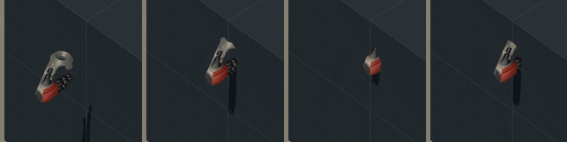
\includegraphics[width=\textwidth]{Sequences/FiltersNone/Seq_FiltersNone.png}
\caption{Sequence showing hand without filters entering obstacle. A gif can be found here: \url{https://tinyurl.com/FiltersNone} .}
\label{fig:filtersNone}
\end{figure}

\begin{figure}[H]
\centering
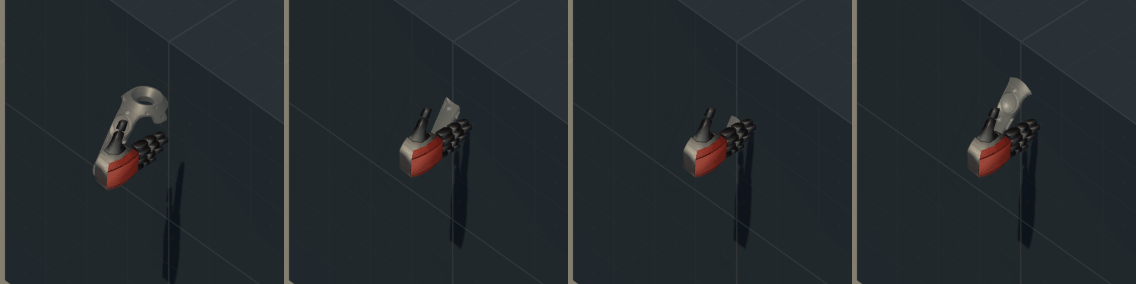
\includegraphics[width=\textwidth]{Sequences/FiltersPosition/Seq_FiltersPosition.png}
\caption{Sequence showing hand filtering on position. Notice that while the hand stays the controller continues to move into the obstacle. A gif can be found here: \url{https://tinyurl.com/FiltersPosition} .}
\label{fig:filtersPosition}
\end{figure}

Implementing position filtering for hands is about determining how to make the hand follow the controller. All of our five prototypes use position filtering, but the implementations of the filters differ. The first distinction is between physics based and non-physics based methods. The Physics Hand is the only one of our prototypes that falls into the first category. The way the Physics Hand is moved towards the controller is to set the velocity each frame so that the hand will reach the controller within the next frame using the physics system. Using velocities and the physics system to move the hand has several positive aspects. The main gain of using the physics system to move is that it adheres to the rules of the system, including collisions, which means that the hand will not penetrate objects in the world which have colliders. One of the downsides of using the physics system to handle collisions and more is that we as the developers have no direct control over the inner workings of the system and therefore lose some control of how the hand behaves.

As for the prototypes that are implemented using non-physics based methods, their filters are all based on three different approaches to stop the hands from penetrating objects: Sweep and place, skip movement in direction and depenetration. These three methods fall into two categories; pre-collision correction methods and post-collision correction methods. The first two methods fall into the pre-collision correction category, because they try to avoid penetration of objects before it happens, whereas depenetration, which falls into the post-collision correction category, will correct the penetration after it has happened. In the different prototypes these three methods are used alone or in combination to create the behavior wanted from that prototype. The simplest of these prototypes is the Rigid Hand. Here only depenetration comes into play. Depenetrating the hand from an object means to find the direction and distance in which to move the colliders of the hand in order for the hand and the object not to be overlapping anymore. The direction and distance are found by finding the minimal translation required to separate the hand from the object. When moving the hands in this prototype, their position is simply set to the target position on the controller each frame after which they are depenetrated from any objects they would be overlapping with. Since the hand is always depenetrated to the closest surface there is a problem of the hand jumping between surfaces, when the controller is moved around inside immovable objects, for instance. If the hand is closer to one surface in one frame and another surface in the next, depenetrating the hand from the object will lead it to the hand switching surfaces, creating a jump.

The problem of jumping between surfaces, when using depenetration is what the Sliding Rigid Hand is trying to solve. It employs the other two methods, Sweep and place and skip movement in direction, in order to combat the jumping . The main idea behind this prototype is to try avoiding penetrating an object altogether or if it happens to only penetrate a small amount so that depenetrating the hand would always select the surface from where it entered the object. Sweeping is about taking the hand and calculating how far in a direction it can move before it hits something. Before moving the hand to the controller position we can sweep and see if it would hit an object on the way. If an object was hit then the hand can be placed there instead of placing it at the controller. This way the hand will not penetrate the object although the controller is inside or on the opposite side of it. In Unity sweeping in a direction will not detect an object if the hand already touches the object. Therefore, in subsequent frames from placing the object on the surface, another method is needed for the hand to not penetrate the object. Skipping movement in a direction is one way to alleviate this problem. When the hand is touching the surface of an object, it shouldn't move in the direction towards the surface, because that would lead the hand to penetrate the object. Therefore, we skip all movement along that direction, essentially allowing the hand to only move on a plane. Moving on a plane works wonders, when interacting with cubes, but has its downsides, when dealing with objects with other shapes. Sliding on a plane might lead the hand to penetrate parts of an object that point out or penetrate other objects. Depenetration helps correct the hands in the situations, where they end up inside an object because correcting in one way leads to errors some place else. These three methods combined should lead to hands that don't penetrate objects, but also doesn't jump between surfaces due to depenetration.

The two remaining prototypes, the Finger Rigid Hand and the Rotation Hand, both use the methods mentioned above to achieve their position filtering. The Finger Rigid Hand use the exact same position filtering method as the Rigid Hand and the Rotation Hand use a filter similar to the Sliding Rigid Hand with the exception that it doesn't do any depenetration.

\subsection{Rotation Filtering}
\label{subsec:categoryRotationFiltering}
To use a rotation filter is to deviate the hands rotation from the current orientation of the controller. In certain contexts it can be beneficial to filter on rotation for the hand to seem more alive and realistic. Hands can adapt their rotation in several ways and different approaches might be taken depending on the context. When approaching a wall with their hand a player's intention in the real world might be to place their hand flat on the wall (palm first). This behavior, where the rotation is adjusted to make interacting with walls more natural, can be implemented using a rotation filter, which takes effect when the hand is approaching a surface.

Another reason to use rotation filtering is to avoid penetrating objects. Besides being an example of how the hands could feel more natural when approaching walls, the reason for rotating the hand to be palm first when getting close to the surface could also be to avoid penetrating the wall. When the hand rotates, the fingers are rotated away from the wall as well, letting the hand get closer to the wall before it starts penetrating it. Using rotation filtering as a means of avoidance also has the goal of reducing the amount of position filtering needed, by allowing the hand to get closer to the controller position, while still being constrained by objects in the world. Rotation filtering is also a big part of pose snapping, which was mentioned Section \ref{sec:stateOfTheArt}. Pose snapping can be used to show available interactions, for instance in Figure \ref{fig:wilsonGrab} from Wilson's Heart, where the hands snap to a pose when they near the suction cups attached to the player's head. Pose snapping of course works much better in unison with both finger position filtering and position filtering. None of our prototypes have explored pose snapping.

The first of the two figures below (Figure \ref{fig:filtersRotation}) shows an image sequence of a hand using only rotation filtering and the second figure (Figure \ref{fig:filtersPositionRotation}) shows an image sequence of a hand using both position and rotation filtering where the rotation filtering is implemented as in the example from above, palm-first towards the surface. It should be noticeable that in the first sequence in the last frame, the hand has entered the obstacle. Using rotation filtering allowed the hand to move closer to the surface before it started penetrating it, but it doesn't stop it completely. Combining the rotation filter with a position filter has the effect of completely stopping it from penetrating the obstacle, while having a more natural look and allowing the hand to get closer to its target.

\begin{figure}[H]
\centering
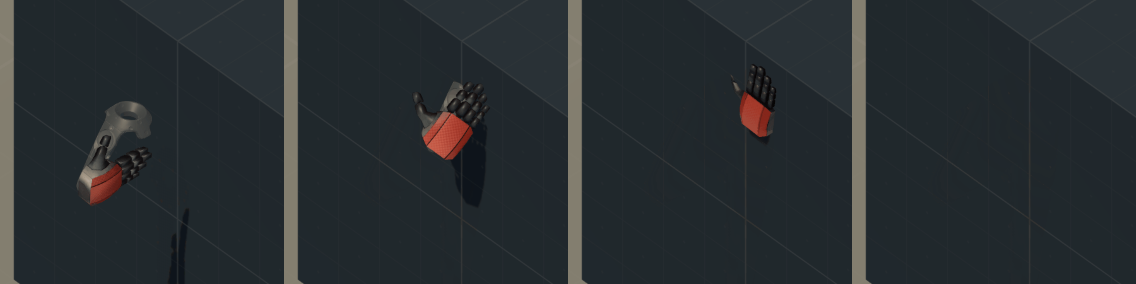
\includegraphics[width=\textwidth]{Sequences/FiltersRotation/Seq_FiltersRotation.png}
\caption{Sequence showing hand filtering on rotation. In the last frame the hand has penetrated the obstacle. A gif can be found here: \url{https://tinyurl.com/FiltersRotation} .}
\label{fig:filtersRotation}
\end{figure}

\begin{figure}[H]
\centering
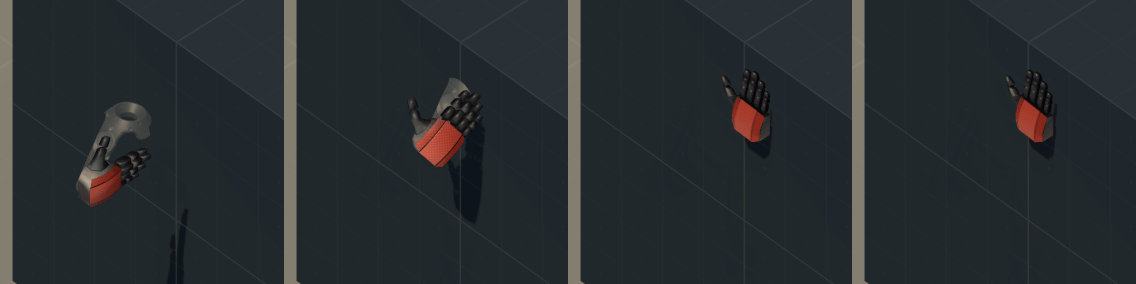
\includegraphics[width=\textwidth]{Sequences/FiltersPositionRotation/Seq_FiltersPositionRotation.png}
\caption{Sequence showing hand filtering on both position and rotation. In the last frame the hand stays on the surface. A gif can be found here: \url{https://tinyurl.com/FiltersPositionRotation} .}
\label{fig:filtersPositionRotation}
\end{figure}

Although all our hand prototypes use position filters, only two of our five hand prototypes (Physics Hand and Rotation Hand) use rotation filtering.

For the physics hand, we don't use any explicit rotation filtering. The physics system decides the rotation of the hand, when interacting with surfaces. While the controller is within an object, the physics hand can decide to rotate the hand to a flat position (either facing the surface with the palm or with the back of the hand) in order to reduce the position deviation between the hand and the controller. The rotation happens as a jump and not as a smooth movement towards the surface resulting in a less natural feel during the jump, but a more realistic look afterwards. To improve upon this, explicit rotation filtering could be added to smoothly rotate the hand to lay flat on the surface, which might remove the jump altogether, but at the same time introduce complexity to the implementation.

Contrary to the Physics Hand, the Rotation Hand uses explicit rotation filtering. The goal of the rotation filtering for this hand is to always approach a surface palm-first. The main example to explain this choice is when the hand approaches a wall. When a player wants to put their hand on a wall, which way would they want to do this? Having an open hand and moving the hand fingers first wouldn't make much sense. It would not give support if the reason for touching the wall was to lean against it, for instance. Rotating the hand so that the palm would be placed firmly on the surface of the wall would make more sense in this case. With this as the main idea behind the rotation, the implementation then had to support this in several cases. The easy case is when the player approaches the wall with an open hand and the palm facing the surface and the back of the hand pointing away from it. Depending on the distance to the surface we rotate the palm of the hand from the controller orientation until it is directly facing the surface. Another case is what to do when the hand is closed into a fist. In this case, the player is probably trying to punch the wall, which means that the palm shouldn't be facing the wall. Testing for this case isn't necessarily hard in itself, but other case can be piled on top of this, including what to do when approaching with the back of the hand, what to do when the player is rotating while the hand is touching the surface and more.

\subsection{Finger Position Filtering}
\label{subsec:categoryFingerFiltering}
Above is mentioned that the player can control the fingers of the hand by pressing the trigger button on the controller. The hand prototypes all have animations that allow them to be either open or closed into a fist. When filtering on the finger positions the target positions of the fingers, or where we want to place the fingers, deviates from the location indicated by the closed value of the hand.

There are two main reasons for wanting to filter the finger positions. The first reason is relatable to the reason to filter on position; we want the fingers and the hand in general to avoid penetrating objects. By bending the fingers when approaching a surface of an object the hand can move closer to the surface before it starts penetrating, for instance, which reduces how much position filtering is needed. Furthermore, the fingers might also bend individually, which can be especially noticeable around edges of objects. Our Finger Rigid Hand and Rotation Hand uses finger position filtering to avoid penetrating objects. The other reason for wanting to filter on finger positions is about indicating whether an object hovered over is interactive or not. In Job Simulator, the fingers bend slightly when the hand is within range of an object that can be grabbed, but they all bend the same amount, though, making the hand look stiff and robotic. The fingers can of course be filtered individually, which can put the hand in a pose that looks like the hand could be stroking the surface or getting a grip the object. Moving the fingers individually makes the hand look much more realistic in its interaction with objects. This approach has been explored with the Physics Hand, which filters on finger positions to show when the hand is hovering over a grabbable object\footnote{A grabbable object is an object which has our grabbable component attached to it. The grabbable component will be described in further detail in section \ref{sec:grabbingSystem} about our grabbing system.} and is close enough to grab it as well. Furthermore, by bending the fingers towards the surface of the grabbable object when approaching it, the Physics Hand allows the player to do things like petting or stroking across object surfaces in a way that looks more natural than with a completely open hand, as can be seen in Figure \ref{fig:strokingFingerExample}.

\begin{figure}[H]
\centering
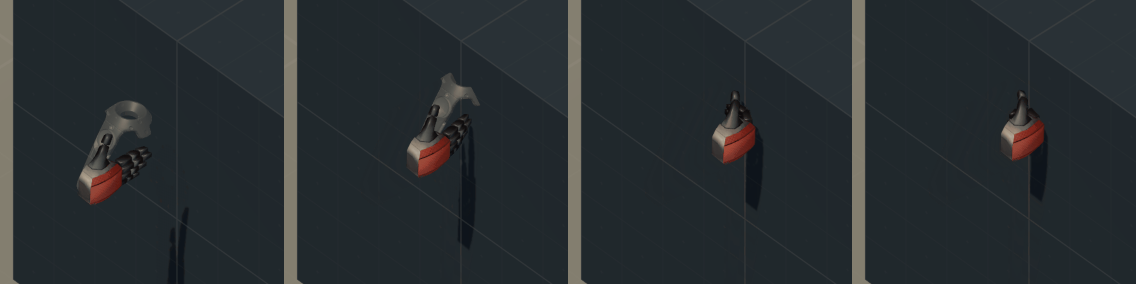
\includegraphics[width=\textwidth]{Sequences/FiltersPositionFingers/Seq_FiltersPositionFingers.png}
\caption{Sequence showing hand filtering on both position and fingers. A gif can be found here: \url{https://tinyurl.com/FiltersPositionFingers} .}
\label{fig:filtersPositionFingers}
\end{figure}

\begin{figure}[H]
\centering
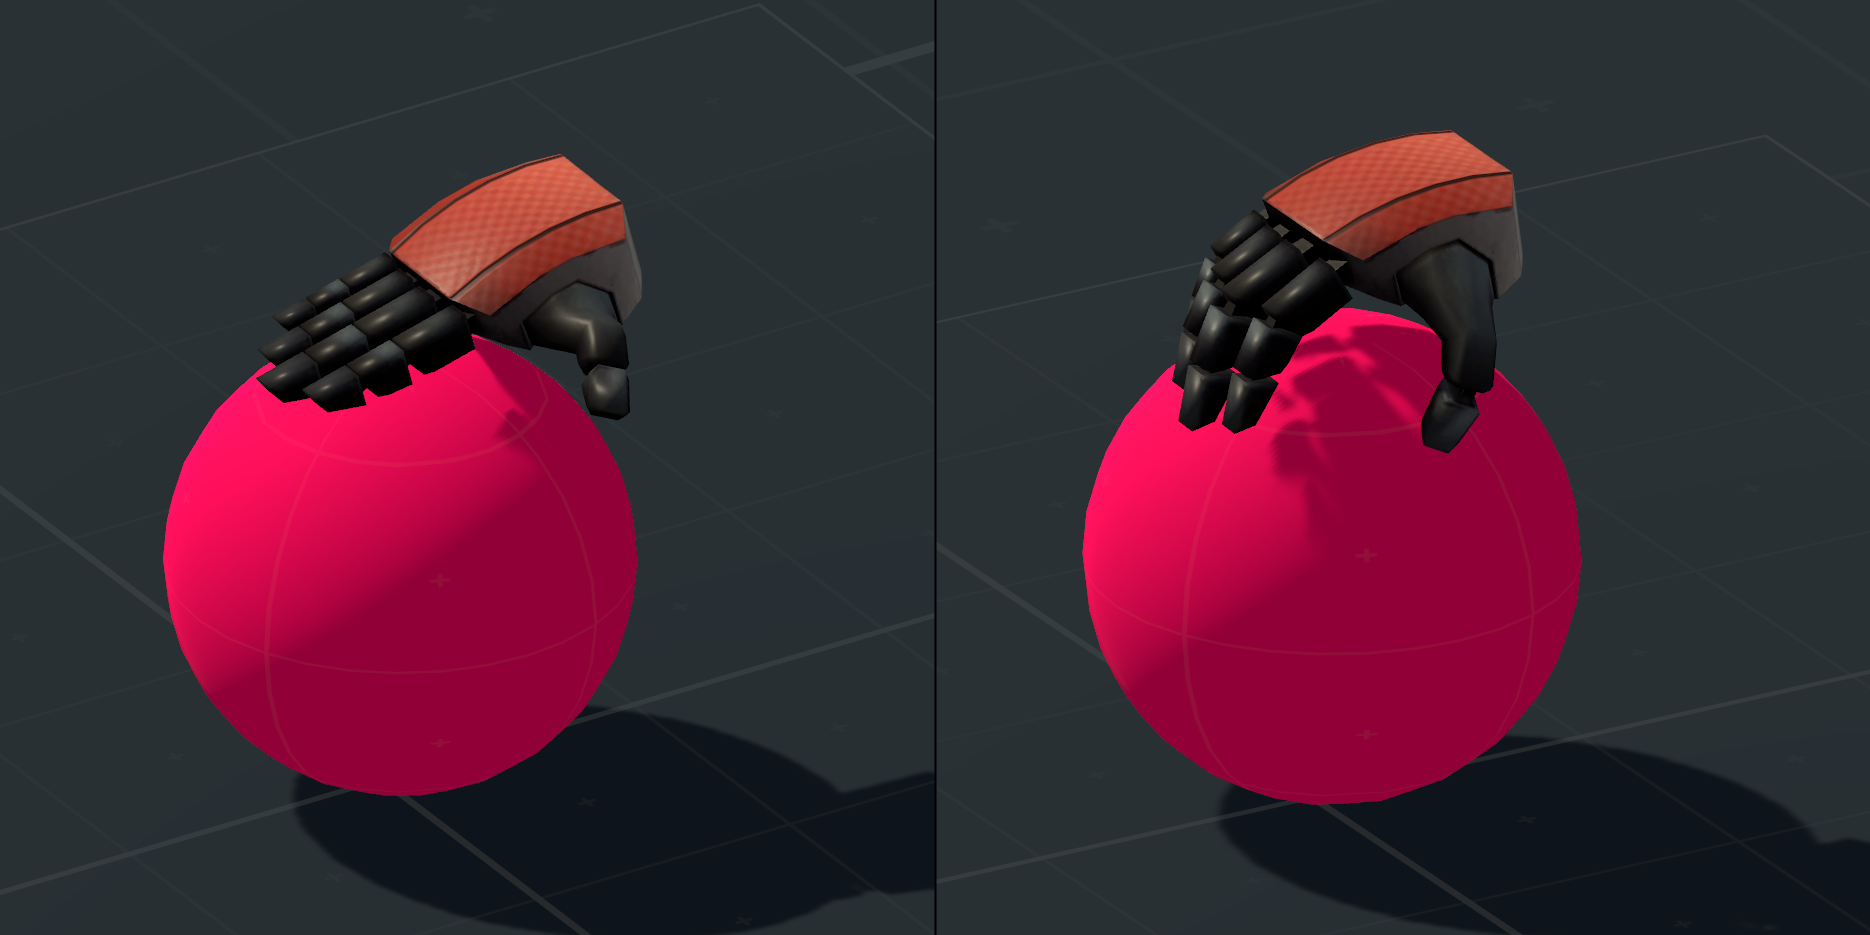
\includegraphics[height=4.5cm]{strokingObject.png}
\caption{Example of petting or stroking object first without and then with finger filtering.}
\label{fig:strokingFingerExample}
\end{figure}

The three hand prototypes that implement finger filtering (the Finger Rigid Hand, the Physics Hand and the Rotation Hand) do so in two different ways. The method used for the Finger Rigid Hand tries to find a suitable closed value for each finger. Each finger can then be animated using this value and its corresponding animation mask. Animation masks are used to isolate a part of the animation data, which makes it possible to use the same animation as for the other hands, while being able to animate each finger individually. The other two hand prototypes make use of an inverse kinematics system (or IK system). Inverse kinematics make use of the kinematics equations to calculate positions for a joint system where we have desired positions for the end effectors. This maps nicely to the movement of fingers, since a finger is a system of joints, where we know the root position of the finger and we'll set the desired location of the end effector, the tip of the finger. The IK system can then calculate how to bend each of the finger's joints to make the tip reach the desired position. To make sure the fingers bend naturally, restrictions can be set for how the joints can bend. The IK system will try to get the tip of the fingers as close to their desired locations as possible without compromising the restrictions for the joints. The restrictions for the fingers are set up in such a way that the joints can only bend around a single axis which means that they cannot bend sideways, for instance. The axis around which they bend is chosen such that bending the fingers closes the hand into a fist. All fingers bend around the same axis, except for the thumb, because of its placement on the hand. We have used a Unity asset pack called Final IK \parencite{RootMotion2017}, which implements several components and methods that can be used to setup and run IK calculations. To move the fingers using the IK system, we move the IK targets, which are the desired locations for the fingertips.

Without going into too much detail about the implementation of the prototypes before Section \ref{sec:handPrototypes}, it's worth mentioning that finding the adjusted closed value for the fingers in the first method and the position for the IK targets in the second involves depenetration of either the hand as a whole or depenetration of individual fingers as well as raycasting to the surface of nearby objects to find locations to place the IK targets and more.

\section{The Hand Prototypes}
\label{sec:handPrototypes}
This section will go into depth about how each of the five hand prototypes have been implemented, mention the pros and cons of the different approaches and finally a step-by-step process for creating the behavior of the prototype will be presented. The table below (\ref{tab:handPrototypes}) stands as a reminder of what filters each of the hand prototypes implements.

\begin{table}[H]
\centering
\caption{The hand prototypes and their filters.}
\label{tab:handPrototypes}
\makebox[\textwidth][c]{
\begin{tabular}{C{2.8cm}|C{2cm}C{2cm}C{2cm}C{2cm}C{2cm}}
 & Rigid Hand & Sliding Rigid Hand & Finger Rigid Hand & Physics Hand & Rotation Hand \\ \midrule
Position filter & \Large X & \Large X & \Large X & \Large X & \Large X\\ \midrule
Rotation filter & & & & \Large X & \Large X \\ \midrule
Finger position filter & & & \Large X & \Large X & \Large X 
\end{tabular}
}
\end{table}

The hands all have a couple of things in common. First the hands require that colliders are set up for their models. We use one box collider for the palm of the hand and one for each part of the fingers, except for the Rotation Hand, which only has colliders on the fingertips and the palm. It's important to make sure that the colliders are not able to collide and interact with each other. In Unity we made all game objects in the hand reside on the same layer (but not the default layer) and made the physics system ignore interactions between objects within that layer. If this is not done, the hand might collide with itself and disallow fingers from bending etc. For the physics hands this is taken one step further where each hand, left and right, has their own layer. The second thing we've used for all hands is Unity's rigidbody component. This component lets the hands interact with the world through the physics system. In Unity a rigidbody component can be kinematic or non-kinematic. A kinematic rigidbody is not affected by outside sources which means it's not affected collisions by, for instance. A non-kinematic rigidbody is affected by outside sources and will be affected by, for instance, gravity and collisions. All of our hands use kinematic rigidbodies with the exception of the physics hands. The last thing the hands all need is an animation to close the hand. Our animations consist of two frames; one where the hand is fully open and one where the hand is closed. We can blend between the two frames using the trigger value from the controller, which therefore controls how closed the hand is. Some of the hands have different considerations whether the hand is open or closed. For all hands we consider the hand closed, when the trigger value - which can be between 0 (not pressed) and 1 (fully pressed) - is equal to or greater than 0.5.

Another thing worth mentioning before continuing to the implementation details for each of the hand prototypes is what the target position and rotation of the hand is. The placement of the hand compared to the controller is a decision that impacts how the user will move the controller around to interact with objects and how the hand feels to use. We chose to place the hand compared to the controller in the virtual world in the same way the user's real hand is placed according to the controller in the real world. As shown in Figure \ref{fig:handControllerPlacement}, the right hand is placed to the right of the controller in a position that could grab and hold the controller. The left hand goes on the left side of the controller but is otherwise the same as the right hand. Our reasoning behind this choice was to map the hand as closely to the position of the user's hands in the real world. From now on, when the controller's position and orientation is mentioned, it's the position and orientation the hands display in this image that we're referring to.

\begin{figure}[h]
\centering
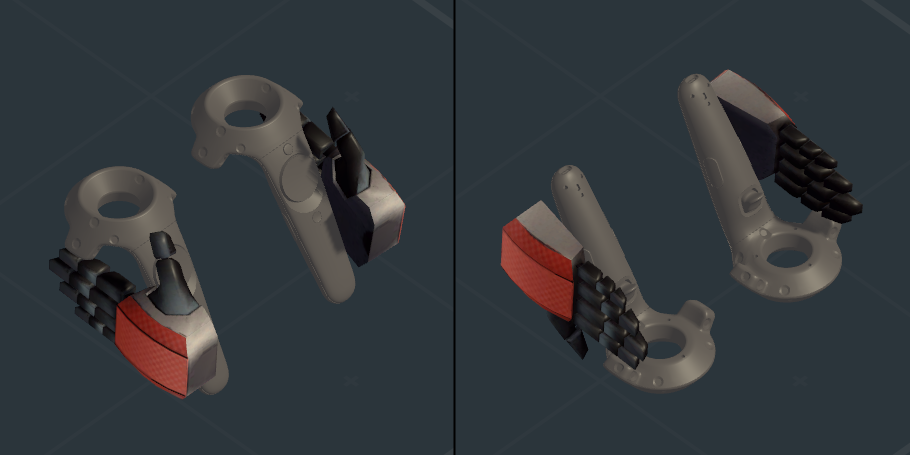
\includegraphics[width=0.85\textwidth]{HandControllerPlacementBoth.png}
\caption{Two images showing the placement of the hands compared to the controllers.}
\label{fig:handControllerPlacement}
\end{figure}

\begin{figure}[h]
\centering
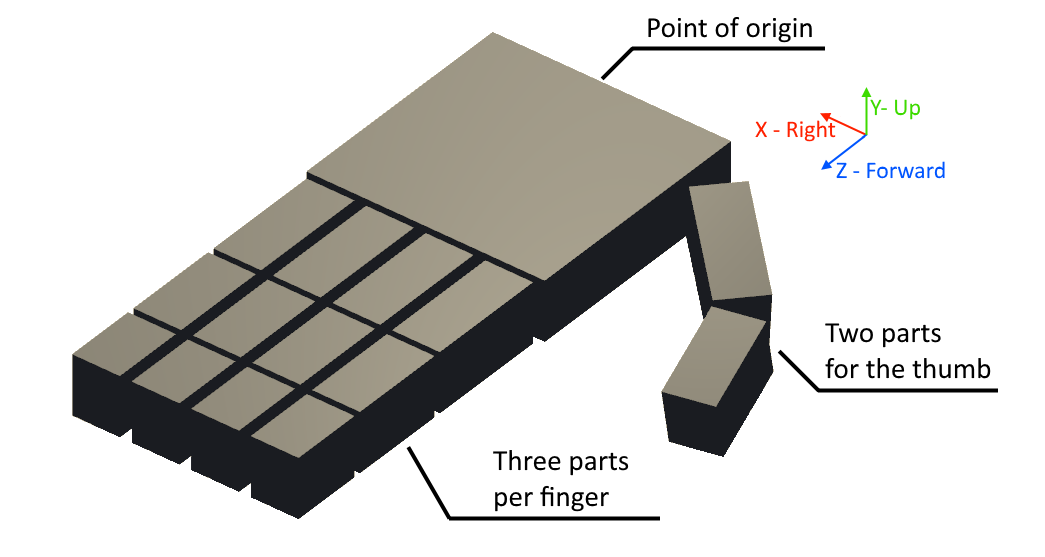
\includegraphics[width=0.85\textwidth]{HandDiagram.png}
\caption{Diagram showing the setup of the hand.}
\label{fig:handDiagram}
\end{figure}

\subsection{The Rigid Hand}
\label{subsec:rigidHand}
As mentioned above in section \ref{subsec:categoryPositionFiltering}, the Rigid Hand moves by setting the rigidbody's position and rotation to the selected position and rotation on the controller. This is done using the $Rigidbody.MovePosition$ and $Rigidbody.MoveRotation$ methods exposed by Unity. Using these methods instead of setting the position and rotation properties directly ensures a smooth rendering in intermediate render frames in Unity and is recommended, when moving a rigidbody, which shouldn't "teleport" \parencite{UnityMovePosition2017}. In the case of moving the hand freely around without any collisions occurring the hand just follows the controller. In the case where the hand has penetrated one or more objects we will depenetrate it from the object. To detect if the hand needs to be depenetrated, we need to check if there is an overlap between the hand's colliders and any other colliders in the world. To reduce the number of colliders to check, we first find all colliders within a radius of the hand. Having these colliders we can now check if any of the hand's colliders have penetrated one or more of them. Unity's Physics API allows us to compute the penetration\footnote{To compute the penetration we use Unity's $Physics.ComputePenetration$ method.} between two colliders, which gives us the depenetration distance and direction. The direction and distance is defined by computing the minimal translation needed to move the collider out of the penetrated object. Iterating over all colliders in both the hand and the penetrated object, we can use the information gathered to move the hand out of the object, correcting the penetration error. The moving and rotation of the hand happens in Unity's fixed update step, which happens at a fixed interval and before the physics simulations. The depenetration of the hand happens in the update step, which happens after the physics simulation. This allows the physics simulation to act upon the situation, where the hand is inside a dynamic object and push it away from the hand. Even though the Rigid Hand is kinematic and is not influenced by outside forces, the dynamic objects are and will therefore try to move out of situations, where their collider overlap with others'.

\begin{figure}[H]
\centering
\small
\begin{enumerate}[noitemsep]
\item Move the hand's rigidbody to the target controller.
\item Orient the hand's rigidbody compared to the target controller.
\item Find all colliders within a small radius of the hand.
\item Compute if any of the found colliders are penetrated by one of the hand's colliders.
\item Depenetrate the hand based on the penetration information computed in the previous step.
\end{enumerate}
\caption{Step-by-step process for placing the Rigid Hand.}
\label{fig:stepByStepRigidHand}
\end{figure}

The Rigid Hand's benefits lie in its simplicity. Very few things are happening, resulting in a simple but suboptimal solution. No matter the orientation of the hand or the position of its fingers, the hand as a whole is moved outside of any penetrated objects so that it is just touching the surface. This makes for a very stiff and lifeless look, when the hand is moved over a surface. Furthermore, as mentioned above, the compute penetration method returns the direction towards the closest point on the surface, but not necessarily a point on the same side of the object as where the hand entered the object. This leads to the hand jumping between different sides of for instance a cube, when the controller is moved between points that are closer to different surfaces. Other drawbacks are linked to the use of a kinematic rigidbody. Using a kinematic rigidbody means that outside forces do not affect the Rigid Hand. Besides having to do collision checking manually, which the depenetration is used for, it has implications for things like pushing objects and is especially noticeable when pushing dynamic objects into immovable objects, which will react in a very unstable and jumpy fashion, because they are locked between two objects which aren't affected by physics. Pushing objects will also give no feeling of mass without additional implementations. Usually the mass of the object pushed would be used to create an opposite force enacted upon the hand, giving different masses a different feel. But since the hand doesn't react to outside forces, this difference is not felt.

The Rigid Hand is used as the base for the Sliding Rigid Hand and the Finger Rigid Hand, which both explore additional filtering to improve the overall feel of the hand. The Sliding Rigid Hand tries to do away with the jumping between surfaces occurring due the compute penetration method always returning the direction to the closest point on the closest surface and the Finger Rigid Hand implements finger filtering to reduce the amount of position filtering needed by allowing the hand to move closer to the surface by bending the fingers.

\subsection{The Sliding Rigid Hand}
\label{subsec:slidingRigidHand}
The Sliding Rigid Hand is state based with two different states: Outside and touching. The two states let the hand behave differently and are used in different contexts. In each frame one of these states will be executed. The state which will be executed will be determined in the beginning of the frame depending on information from the last state executed and from the current context.

\todo[inline]{Explain what a frame is. Perhaps in a footnote.}

The outside state is executed, when the hand is not touching an object. When executed the hand is first rotated to the orientation of the controller target. After rotating the hand, we sweep towards the controller, checking if there's any object in between the hand and the controller. If no obstacle was in the way, the hand is moved towards the controller. If an object is blocking the path we then position the hand so that it is touching the object. Unity's $Rigidbody.SweepTest$ method gives us the necessary information to do so: direction and distance to the object that was blocking the path\footnote{The direction and distance found by the $SweepTest$ method is between the closest points between the two objects: The direction and distance between the point on the hand that is closest to the closest point on the object hit.}.

There is only one transition from the outside state to the touching state; if the sweep detected an object in between the hand and the controller, while executing the outside state, the hand will have been placed on the surface of the object. In this case we will switch to the touching state. If nothing was obstructing the path the hand stays in the outside state.

As with the outside state, the first thing that happens in the touching state is that we rotate the hand so that it matches the orientation target on the controller. Because we rotated the hand while it was touching an object, we need to check two things; if the rotation has resulted in the hand having penetrated the object or if the rotation has caused the hand to be removed from touching the surface of the object. First, we check if the hand is inside an obstacle and depenetrates it if necessary. This is done in the same fashion as mentioned for the Rigid Hand (Section \ref{subsec:rigidHand}). If the hand wasn't inside any object we try to sweep towards the controller position to check if the hand is currently not touching any object. If the sweep resulted in hitting an object in the path towards the controller, we move towards the location hit on that object. This works like mentioned in the outside state above with one small addition. We need to save the normal of the point where the hand touches the surface. When we use Unity's $Rigidbody.SweepTest$ method we gain some information about the object hit, if any. This includes the normal of the point on the object hit by the sweep. We need this normal for the next part: Sliding. Sliding is where we skip movement in a particular direction (and its opposite), effectively moving the hand on a plane. In this case, we skip movement along the normal and its opposite. An example of sliding in use is when the hand is interacting with a flat surface and the controller is inside the surface. When moving the controller around inside, the hand should slide on the plane created by the normal of the contact point, which is approximately the same as sliding across the surface, if the contact point is updated frequently. To implement the sliding we first find the vector between the hand and the target on the controller. This vector is projected onto the plane created with the normal. Moving the hand along this new projected vector reduces the distance to the controller without penetrating the object. As a final step for the touching state, the hand is depenetrated again to make sure it's not inside an object after sliding. To summarize, the touching state rotates the hand and then checks if the hand has now been removed from or placed inside an object and if it has, it's moved to the position where it's touching again. Afterwards the hand then slides to the position on the plane created by the normal which is the closest to the controller.

There are two transitions from the touching state back to the open state. The first transition checks if the controller has moved back outside the object compared to the surface the hand is currently touching. The direction from the hand's current position to that of the controller is computed. If this direction is in the same general direction as the normal of the surface\footnote{To determine if the direction vector points in the same general direction as the normal, we use the dot product of the two. If the dot product is positive they are pointing in the same general direction.}, it means that the controller was moved back outside the object in the direction from where it entered. In this case the hand goes to the outside state. The other transition checks if we can sweep with the hand to the controller. If we can sweep all the way without hitting any objects it means that the hand has slid over an edge and the controller is currently free of any objects. Due to how Unity's $Rigidbody.SweepTest$ method is implemented, it's necessary to move the hand slightly away from the object's surface when sweeping. This is due to the fact that when the object is touched, sweeping doesn't recognize the object being hit. We therefore move the hand slightly back in the direction of the normal of the contact point, before sweeping, but reset the position again when the sweep has been performed. In the case we hit something, the hand is still touching a surface and we stay in the touching state. If not the hand transitions into the outside state.

\begin{figure}[H]
\small
\begin{enumerate}
\item Transition to new state, if necessary.
\begin{enumerate}[noitemsep,label=\alph*.]
\item If the last state executed was outside, transition to the touching state if:
\begin{enumerate}[noitemsep,label=\arabic*.]
\item the sweep during the last outside state execution hit an object.
\end{enumerate}
\item If the last state executed was touching, transition to the outside state if:
\begin{enumerate}[noitemsep,label=\arabic*.]
\item the controller was moved away from the currently touched surface (in the general direction of the normal of the contact point), or
\item the sweeping towards the controller didn't hit any object.
\end{enumerate}
\end{enumerate}
\item Execute selected state behavior.
\end{enumerate}
% first column
\begin{minipage}[t]{0.49\textwidth}
\small
The outside state:
\begin{enumerate}[noitemsep]
\item Orient the hand's rigidbody compared to the target controller.
\item Sweep towards the target controller.
\item If no obstacles in the path between the hand and the controller, move the hand's rigidbody to the target controller.
\item Else move to the position where the sweep hit the obstacle.
\end{enumerate}
\end{minipage}
\hspace{2em}% <---- Don't forget this %
%second column
\begin{minipage}[t]{0.49\textwidth}
\small
The touching state:
\begin{enumerate}[noitemsep]
\item Orient the hand's rigidbody compared to the target controller.
\item Check if inside object and depenetrate if so.
\item If the hand was not inside an object, sweep towards the target controller.
\item If the sweep hit an object, the controller was not touching. Position the hand on the object hit using the sweep information.
\item Use the normal of the contact point to define a plane on which to slide to minimize the distance to the controller.
\item Check if sliding the hand has led it to penetrating an object and depenetrate if so.
\end{enumerate}
\end{minipage}
\caption{Step-by-step process for placing the Sliding Rigid Hand.}
\label{fig:stepByStepSlidingRigidHand}
\end{figure}

\todo[inline]{Maybe split the sliding rigid hand step-by-step figure into two figures, so it can be split over two pages.}

What the Sliding hand tries to solve, using the above described state based approach is to remove the jumping created by using only depenetration. This flaw is very evident with the Rigid Hand, as the controller moves around inside objects. Since depenetration always moves the hand to the closest point on the surface of the object it's depenetrating from, the main idea of the Sliding Rigid Hand is to never allow the hand to penetrate deeply enough to select another surface than the one it entered from. This means that unlike the Rigid Hand, where the position is updated every frame to the controller target, we always sweep and place, while in the open state, which disallows penetration altogether. Therefore the touching state is the only place where the hand can move or rotate into a position, where it penetrates an object. But because of the restriction of movement along the normal of the contact point, the hand never penetrates the object very far, resulting in the depenetration selecting the same surface even though the controller might be closer to another.

This approach works extremely well on flat surfaces, where the plane created by the normal will be approximately the same as the actual surface the hand is touching, but difficulties arise with non-flat surfaces like curved, rough and concave shapes. Depending on how often the normal is updated, the plane defined by it isn't a very good approximation of the surface, which can lead the hand to not stick to the surface, when moving across it. In our implementation, the normal is only updated upon sweeping, which happens in both states, but only when the hand has been found to be outside the object. The information gathered during depenetration doesn't help much, since the methods for computing the penetration in Unity doesn't give any information about the normal of point of the surface to which the hand would depenetrate, which puts us in a position, where we don't update the normal often enough to handle situations like curved shapes properly. This could be improved upon by finding ways to reliably update the normal of the current contact point more often, which could include sweeping every frame to find the normal during the touching state, for instance. Besides these problems, the same troubles concerning the kinematic rigidbody are inherited from the Rigid Hand, leaving us with a hand that works quite well in a low number of situations, which restricts the use cases in which the Sliding Rigid Hand would perform satisfactory.

\subsection{The Finger Rigid Hand}
\label{subsec:fingerRigidHand}
The Finger Rigid Hands are based upon the Rigid Hand's way of moving and rotating, but tries to improve upon it by adding finger filtering on top. Where the Rigid Hand moves and rotates using the rigibody's $MovePosition$ and $MoveRotation$ methods and then depenetrates the hand from possible overlaps with objects in the world, the Finger Rigid Hand adjusts the fingers in between the placement and the depenetration.

Before continuing with how the Finger Rigid Hand and its fingers are placed, we need to mention that the animation for this hand is a bit different from the other prototypes. The animation for the Finger Rigid Hand has a mask for each finger, which means that the fingers can be animated individually even though we use the same animation frames as for the other prototypes, namely one open and one closed hand frame.

As mentioned above the first thing the Finger Rigid Hand does is to move to the location of the orientation of the controller by using its rigidbody's $MovePosition$ and $MoveRotation$. When the hand has been placed we save the current closed value of each finger. The closed value here isn't necessarily the same as the trigger button value\footnote{As mentioned above, the trigger button on the controller is mapped to the closing of the hand, by using its value to blend between the open and closed animation frames.}, as this is how closed the finger was after the adjustment last frame. After saving the closed values all the fingers are opened fully using the animation. We need to do this before the next step, which is to calculate the average up vector of all the finger parts for each finger. So for each finger, the average over all its parts' up vectors is saved. When the averages have been calculated, we reset the fingers' closed value to the value saved before and the finger positions are updated according to their closed value using the animation. The next step is to depenetrate the hand from any nearby objects, which is done as previously described. This step is important because we're going to raycast from the fingers later and we need to make sure the origin of the raycasts aren't inside any objects we would like to raycast towards\footnote{In Unity raycasts don't hit backfaces of object models, so to be sure that the raycast hits the object at the correct position, the origin needs to be outside of the object.}. 

With all this legwork done, we're now set to start adjusting the fingers. The general idea is that we want to find out how the fingers are oriented according to the surface they are interacting with. There are three cases we consider for each finger: If the hand is not near any objects, the finger doesn't adjust, if the hand is positioned such that bending the finger will not allow it to move away from the surface (the rotation axis is parallel to the surface normal), we skip adjusting the finger and the last case is if the rotation axis is not parallel with the surface normal. In this case we use the difference between the normal and the rotation axis to decide on how to adjust the finger.

Before we go into the calculations for the individual fingers we first calculate the distance between the hand and the controller. All the fingers use this value to calculate with how much to adjust. With the distance calculated the next steps are performed per finger. To find out if a finger's rotation axis is parallel with the surface normal, we first find the colliders within a radius of the hand\footnote{Unity's physics API exposes the method $Physics.OverlapSphere$ for finding all colliders within a certain radius from a point.} and find the one closest to the finger. If no collider was found near the hand, we skip the finger adjustment and lerp its closed value towards the value determined by the players input. If a collider was found, we use raycasting to find the normal of the closest point on the collider\footnote{The closest point on a collider can be found using Unity's $Collider.ClosestPoint$ method.}. Since we defined the rotation axis of the finger ourselves and we found the normal of the surface, we can take the dot product of the two to see if they are parallel with each other. If they are, the finger cannot bend away from the surface and like with the case of no nearby colliders the finger's closed value is lerped towards the closed value defined by the player's input. In the final case where the normal and the finger's rotation axis are not parallel, we use the dot product between the normal and the average up vector we calculated earlier and the distance from the hand to the controller to find the value with which to adjust the finger's closed value by. We don't use these two values directly, but feed them each to one of Unity's animation curves\footnote{Unity's animation curves are functions that can be visually defined and takes an input value and returns an output value.}: One that evaluates the distance and one that evaluates the dot product. The two resulting values are then multiplied with each other, giving us the adjustment for the finger. After calculating the adjustment value for the finger, we set the finger's closed value equal to the sum of the closed value defined by the player's input and the adjustment value. When all the fingers' closed values have been set, they - along with the animation masks - are used to update the animation of the hand.

As the final thing after having adjusted the fingers, we again want to move the hand to the controller's position\footnote{We only need to move the hand, not rotate it, because depenetrating the hand doesn't rotate it.} and then depenetrate a final time. The reason to this is because having depenetrated and adjusted the fingers might lead to the hand not being positioned at the controller while also not touching the surface of an object. The hand should only be separated from the controller's position, when the hand can't reach it because there's an object in the way. By moving once more and depenetrating we make sure that the hand is placed at either the controller's position or on the surface of the object the controller is inside.

\begin{figure}[H]
\centering
\small
\begin{enumerate}[noitemsep]
\item Move the hand's rigidbody to the target controller.
\item Orient the hand's rigidbody compared to the target controller.
\item Find the average up vector for each finger:
\begin{enumerate}[noitemsep]
\item Open the finger.
\item Take the average of the up vectors of each part of the finger and save it.
\item Move the finger back to the previous position.
\end{enumerate}
\item Depenetrate the hand from any object it might have entered after moving and rotating.
\item Calculate the distance from the hand to the controller.
\item Calculate the adjustment value for each finger and apply it:
\begin{enumerate}[noitemsep]
\item For each finger, find the closest collider within a radius from the hand.
\item If no collider found within range lerp the finger's closed value towards the closed value indicated by the player's input and skip the rest.
\item Find the closest point on the collider found.
\item Find the normal on the closest point of the collider by raycasting to the closest point.
\item If the normal found and the finger's rotation axis are parallel, lerp the finger's closed value towards the closed value indicated by the player's input and skip the rest.
\item Else calculate the dot product between the average up vector of the finger (calculated in one of the previous steps) and the normal.
\item Normalize the distance between the hand and the controller by dividing with a max distance value defined for each finger and clamping the result between 0 and 1.
\item Feed the dot product and the normalized distance into each their animation curve and multiply the results with each other to get the adjustment value for the finger.
\item Set the finger's closed value to the closed value indicated by the player's input summed with the calculated adjustment value.
\item Update the finger's position using each of the finger's closed value and its corresponding animation mask, which allows for animating the fingers individually.
\end{enumerate}
\item Move the hand's rigidbody to the target controller (after depenetration it might have moved away from the controller).
\item Depenetrate the hand after adjusting the fingers and having moved it again.
\end{enumerate}
\caption{Step-by-step process for placing the Finger Rigid Hand and its fingers.}
\label{fig:stepByStepFingerRigidHand}
\end{figure}

As mentioned above, filtering on finger positions can make the hand feel less stiff, when interacting with objects, but it can also be used with the purpose of avoiding penetration. The main goal of this prototype was to experiment with the latter. As described above, the fingers bend when the hand approaches an object and the direction they bend depends on the hand's angle compared to normal of the nearest point on that object. Bending the fingers like this enables the hand to move in closer to the object, before it needs to filter on the position to avoid penetrating the object. Another benefit from bending the fingers, when interacting with objects is that the hands look a lot less stiff than hands that don't filter on the finger positions, especially because the bending is very smooth. It looks and feels more like a human hand compared to a robotic hand, for instance. The Finger Rigid Hand doesn't solve any of the problems that the we mentioned about the Rigid Hand, of which it is based. The Finger Rigid Hand still jumps around an object, when moving the controller around inside the object, due to depenetration selecting the closest point on the object to move to and the troubles introduced by using a kinematic rigidbody also still exist. The addition of adjusting the fingers also introduce some new cases where the hands aren't stable. This prototype doesn't handle edges and corners very well. The fingers behave in strange ways since the sweep of the hand still hit the object even though some of the fingers are free to open fully. At corners the hand can't always decide on the side to depenetrate to, because depenetrating to one side, make the fingers bend in a certain way so that when the hand is depenetrated the next time it's closer to another point on the object, resulting in the hand jumping between several positions around the edge or corner. Again, like with the Sliding Rigid Hand, the Finger Rigid Hand introduces more problems than it solves, although it proves the fact that the feel of the hand in the cases where it works, is very different from the hands that don't have finger filtering.

\subsection{The Physics Hand}
\label{subsec:physicsHand}
The main difference between the Physics Hand and the other prototypes is that it is using a non-kinematic rigidbody and is therefore affected by the physics simulation. This means that it can be pushed around by other objects and the physics system will handle collisions. To properly work with the physics system, the hands need to be moved and rotated differently from the other hands. Instead of setting their position and orientation directly, velocities are applied which makes the hand move and rotate to where they need to go. This means that we calculate what velocity is needed for the hand to move the distance between itself and the controller target and the angular velocity needed for the hand to rotate to the controller orientation. In Unity it's important that these velocities are set in the fixed update method, because they need to be applied before the engine's physics calculations takes place\footnote{Unity's order of execution can be seen from a chart in their online documentation \parencite{UnityExecutionOrder2017}.}. Although this is our own implementation it draws heavy inspiration from how the hands are moved in the NewtonVR asset pack \parencite{TomorrowTodayLabs2016}.

Before applying the velocities described above, we adjust the fingers of the hand. As mentioned above, the fingers of the Physics Hand are moved using an IK system. The Physics Hand has several states that indicate whether the finger positions should be filtered or not. The states are named as follows: Free, Fist, Hover, Holding and Lerp to free. When the hand is not near any objects and the player hasn't closed the hand using the trigger button on the controller the hand will be in the Free state. In this state, the fingers will be positioned according to the animation and the trigger value. The trigger value is used to blend between the open and closed frames of the hand's animation. The animation is used to determine the IK targets' locations. The hand can transition from the Free state into the Fist state, if the player presses the trigger enough for the hand to be considered closed\footnote{As mentioned above, in our prototypes we consider the hand closed when the trigger has been pressed half way, meaning that the trigger value is 0.5 or above.}. In the Fist state the fingers work exactly like in the Free state, dictated by the animation and the trigger value. The reason to have the closed state is to disallow certain transitions that are otherwise possible from the Free state. The Fist state can transition back to the Free state, when the player again opens the hand. Besides transitioning to the Fist state, the Free state can also transition to the Hover state. This happens when there is a grabbable object inside the hand's grab area. The grab area is a trigger collider attached to the hand which indicates the range at which the hand can grab objects in the world. When a grabbable object enters the grab area trigger and the object is below the hand, as in the object is on the side the palm of the hand is facing, the hand enters the Hover state. In the Hover state the finger positions will be filtered in a way that tries to let the fingers approach and touch the object. This filtering will be described further below. From the Hover state the hand can transition to either the Holding state or the Lerp to free state. The Holding state is entered, when the player has grabbed an object. In the Holding state the fingers are not updated, effectively fixating them to their last positions. The hand transitions from the Hover to the Lerp to free state, when there is no grabbable object inside the grab area trigger anymore. The Lerp to free state is inserted in between the Hover and the Free / Fist states to make the transition smooth. In the Lerp to free state the fingers will lerp from their hover positions back to the positions indicated by the animation and trigger button values. When the lerping has finished, the hand will automatically transition to either the Free or the Fist states depending on whether the hand is closed or not. The Free to lerp state can be interrupted if the hand is again hovering over a grabbable object in which case it transitions back to the Hover state.

% Example of tikz automata: http://www.texample.net/tikz/examples/state-machine/

\begin{figure}[H]
\centering
\begin{tikzpicture}[->,>=stealth',shorten >=1pt,auto,node distance=5cm, semithick]

\tikzstyle{every state}=[fill=red!30,draw=black,text=black,minimum size=2cm]

\node[state]				(A)											{Free};
\node[state]				(B) [right of=A]					{Fist};
\node[state]				(C) [below of=A]				{Hover};
\node[state, align=center]				(D) [below right of=A]	{Lerp \\ to \\ Free};
\node[state]				(E) [left of=A]					{Holding};

\path 
(A)		edge	[bend left]		node {1} (B)
			edge								node {3} (C)
(B)		edge [bend left]		node {2} (A)
(C)		edge [bend left]		node {4} (D)
           	edge [bend left]		node {8} (E)
(D)		edge 								node {6} (A)
           	edge								node {7} (B)
           	edge [bend left]		node {5} (C)
(E)		edge								node {9} (A)
			edge [bend left]		node {10} (C);
\end{tikzpicture}
\begin{enumerate}[noitemsep]
\small
\item Hand is closed.
\item Hand is opened.
\item Grabbable object in grab area.
\item No grabbable object in grab area.
\item Grabbable object in grab area.
\item Lerping fingers to closed value has finished and the hand is not closed.
\item Lerping fingers to closed value has finished and the hand is closed.
\item When grabbing object.
\item Object dropped and no grabbable object in grab area.
\item Object dropped and grabbable object in grab area.
\end{enumerate}
\caption{State diagram for the Physics Hand's fingers.}
\label{fig:physicsHandStateDiagram}
\end{figure}

As mentioned above, the fingers positions are only filtered in three of the five states: The Holding state, the Hover state, the Lerp to free state. The Free and Fist states don't filter the input but lets the fingers follow the animation and trigger button value directly. In the Holding state the finger positions are filtered by skipping the input completely. The fingers are fixed, while holding objects. The Hover state is where the most interesting filtering happens. It has several steps to find the positions for the fingers, but first we see if the there is a need to adjust the fingers at all by checking if the grabbable the hand was hovering over is still within the grab area. If not, we skip adjusting the fingers, since in the next frame the hand will transition out of the Hover state, as mentioned above. If there is a grabbable object in the grab area we first place the fingers in accordance to the animation and trigger button value to use as the starting position.

What the Hover state tries to achieve is to find suitable positions on the surface of the grabbable object on where to place the fingers. We try three different methods in priority to find the best location for each finger. The first of the three methods is to find the point on the grabbable that is the closest to the fingertip\footnote{Unity's API allows us to find the closest point on a collider from a given point by using the $Collider.ClosestPoint$ method on the collider in question.}. The next method is to find the point on the surface found by moving along the negative up vector of the fingertip, so finding a point on the object that is directly below the fingertip. For this we use raycasting from the fingertip in the direction of the negative up vector of the fingertip. The final method is to find some direction in between the negative up vector of the fingertip and the direction towards the closest point on the grabbable object. In order to find this middle direction we lerp between the vectors for the direction to the closest point and the negative up vector with respects to a middle interpolation value\footnote{This value is a value between 0 and 1, where 0 returns the start lerping vector and 1 returns the end lerping vector. Using different values moves the position found for the fingers in between the two given direction vectors. We use the value 0.86 for our Physics Hand.}. The last two methods are not guaranteed to hit the grabbable object at all. The priority of the three methods is as follows; first we see if moving along the direction which is in between the negative up and the direction to the closest point hits a point on the grabbable object. If it does, we use that point as the position the finger needs to move to. If it didn't hit, we try with the negative up from the fingertip and if it hits, we use that hit point as the position to move the finger to. If none of the above methods resulted in a point on the grabbable object then the closest point on the object is used as the target for the finger. The reason for this prioritization has to do with how good the fingers look after adjusting them for certain placements of the hand compared to the grabbable object and the grabbable object's shape. If the closest point was always used and the hand was hovering over a grabbable cube with the palm on one of the surfaces and the fingers sticking out over the edge, the result would lead to the two furthest joints in the fingers both bending about 90 degrees without the joint between the fingers and the palm bending much, which is not a natural pose and is therefore not ideal. Figure \ref{fig:physicsHandFingerPlacementDiagram} displays the three directions in a diagram. The same will occur when hovering over thin objects like sticks or bats. The closest position on the grabbable from the fingertips will be close to the palm resulting in the weird pose. Using the negative up vector of the fingertips will also not work in a lot of cases. If we again look at the example with the grabbable cube. If the hand is completely open and the fingers are sticking out over the edge, moving along the negative up vector will not lead to a hit on the cube. Because of this, having a middle point between the closest point and the negative up can help in these cases by bending the fingers towards the grabbable object, but with a more natural pose than what results from the closest point. When the positions for the fingertips have been found by using one of these methods we lerp the IK targets of the fingers towards the found positions, as to smooth out the movement, after which we call the IK system to solve for the new position.

\begin{figure}[H]
\centering
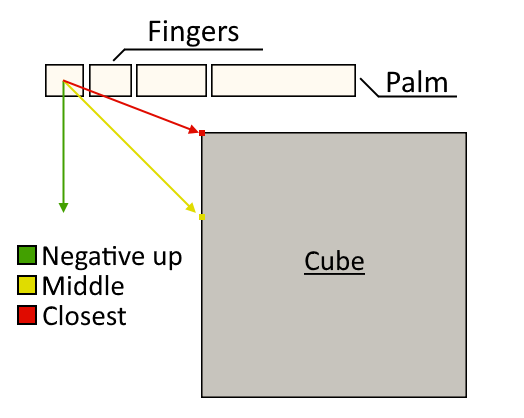
\includegraphics[height=5cm]{FingerWrappingDiagram.png}
\caption{Diagram showing the hand from the side above a cube with arrows pointing in the directions used for finding the locations to place the fingers.}
\label{fig:physicsHandFingerPlacementDiagram}
\end{figure}

\begin{figure}[H]
\centering
\small
% POSITION AND ROTATION.
\begin{flushleft}
Position and rotation:
\end{flushleft}
\begin{enumerate}[noitemsep]
\item Calculate the angular velocity needed to rotate the hand to the orientation of the controller in this frame and apply it to the hand's rigidbody.
\item Calculate the velocity needed to move the hand to the position of the controller in this frame and apply it to the hand's rigidbody.
\end{enumerate}
\caption{Step-by-step process for placing the Physics Hand.}
\label{fig:stepByStepPhysicsHandPositionRotation}
\end{figure}

\begin{figure}[H]
\centering
\small
% FINGER POSITIONS.
\begin{flushleft}
Finger positions:
\end{flushleft}
\begin{itemize}[noitemsep]
\item If in the Hover state:
\begin{enumerate}[noitemsep]
\item Check if there is a grabbable object in the grab area of the hand below the palm. If not, skip the rest.
\item Move all fingers to the location indicated by the animation and the trigger button value as a starting position.
\item For each finger, get the negative up vector from the fingertip.
\item Get the closest position from the fingertip to the grabbable object and create a direction vector starting from the fingertip and pointing at the closest point.
\item Calculate the middle vector as a vector which resides between the negative up and the closest point direction. This can be done by lerping. The amount by which to lerp is a variable which needs to be tweaked.
\item Raycast towards the middle direction with the max distance being the radius of the grab area. If the grabbable object was hit, set the hit point as the finger's target.
\item If the previous raycast didn't hit the object, raycast in the negative up direction with the same distance. If the object was hit, set the hit point as the finger's target.
\item If none of the raycasts hit, use the closest point on the grabbable object as the finger's target.
\item Set all fingers to their open position using the animation as a base. This is to start the IK solving from the same location every frame.
\item Lerp the finger's IK targets towards the calculated finger targets.
\item Let the IK system solve for the new IK targets and move the fingers.
\end{enumerate}
\item If in the Lerp to free state:
\begin{enumerate}[noitemsep]
\item For each finger, save its current IK target position.
\item Get the position that each finger would have according the the animation and trigger button value.
\item Find an intermediate position for the fingers slerping\footnote{SOMETHING ABOUT SLERPING HERE!} from the saved IK target position towards the animation position.
\item Set the IK target of the finger to the intermediate position found for it.
\end{enumerate}
\item If in the Holding state:
\begin{enumerate}[noitemsep]
\item Skip all finger movement.
\end{enumerate}
\item All other states:
\begin{enumerate}[noitemsep]
\item Set each finger's IK target to the position indicated by the animation and trigger button values.
\end{enumerate}
\end{itemize}
\caption{Step-by-step process for placing the Physics Hand's fingers.}
\label{fig:stepByStepPhysicsHandFingers}
\end{figure}

The previously mentioned prototypes all have troubles caused by using a kinematic rigidbody. Collisions must be handled manually and that creates a lot of cases that need to be solved before the hands look really nice, when interacting with objects of different shapes and types. Unity's physics system already handles most of these cases, when two physics objects interact with each other. Therefore, the main idea behind the Physics Hand is to let the physics system handle all the difficulties that arise due to collision handling. But besides handling just collisions, using a non-kinematic rigidbody enables the Physics Hand to do a couple of extra things out of the box, which include lifting and having a sense of weight when interacting with objects. Lifting here means to be able to lift an object without grabbing it using a grabbing mechanism\footnote{All hand prototypes implement a grabbing mechanism, which when activated allows the grabbed object to follow the hand. The different implementations are described below in Section \ref{sec:grabbingSystem}.}, which in our case is activated by pressing the trigger until the hand is closed. An example of how to lift an object using the Physics Hand is to place the left and right hand on either side of an object, push the hands towards the object and then move the controllers upwards. The physics system will use the friction between the materials, the mass and the force with which the hands push into the object to enable the lifting of the object. This also leads into the sense of weight. Since all interactions, collisions included, are now fully physics based it means that the objects the hands interact with are also applying forces to the hands. When trying to lift a heavy object, the player might not be able to and the hands will slide across the surface instead of lifting the object. The sense of weight also applies to the context of pushing, where the hands will be separated more from the controller position, when pushing heavier objects than with lighter objects, which gives a different feel to pushing objects of different weight.

Besides all these good things that comes with the use of a non-kinematic rigidbody, there are also downsides that tag along. The rotation filtering occurring with the Physics Hand is also controlled by the physics system, as with the position filtering, but in some cases it doesn't act in a satisfactory fashion. When placing the hand flat on the surface of an object and then turning the controller, the hand stays flat on the surface, which feels very natural. The opposite of this is when the hand is pushed towards the surface fingers first. At first the hand will look a lot like the Rigid Hand, staying outside the object, but when the controller is far enough from the hand, it jumps to a position where the hand is flat on the surface. This jump feels unnatural. One way to avoid this jump would be to create explicit rotation filtering to handle the cases, where the hand would rotate in a frame and smoothly rotate the hand instead. This problem isn't seen very often, though, since the hand rotates more smoothly, when it approaches the surface at an angle instead of straight on. Along with the rotation jump there are also problems that are related to the moving of the fingers. When the fingers are bend, the rigidbody moves or rotates slightly, which might make is look like it is shaking. Our guess as to why this is happening is that when the fingers are bend the physics system simulates that they exert a force on the surrounding air, which in turn using Newton's third law applies an opposite force back on the hand, making the rigid body move. This moving and rotating of the hand, by only bending the fingers, is not the wanted behavior. The hand should be able to stay still, while the fingers are bending. The way we solved this was by increasing the drag and angular drag of the hand's rigidbody to the point where the movement and rotation caused by bending the fingers wasn't noticeable any more.

\subsection{The Rotation Hand}
\label{subsec:rotationHand}
The Rotation Hand is the only prototype we implemented that explicitly filters on all three variables: position, rotation and finger positions. It has two modes of movement. First, we check if there are no objects in the hand's vicinity. We can do this by using Unity's physics API which exposes the method $Physics.OverlapSphere$ for finding all colliders within a certain radius from a point. If there are no objects nearby the position and orientation of the hand is set to the position and orientation of the controller. If there are object nearby we act upon the closest collider. We first want to rotate the hand. The goal of the explicit rotation filtering is to make the palm face the surface of the object, when the hand is open and make the front of the hand face the surface, when the hand is closed into a fist. These two orientations can be seen in Figure \ref{fig:rotationHandFacingDirections}. The rotation should be more or less complete depending on the distance to the object meaning that if the hand is touching the object, the palm should be facing directly towards the surface and if the hand is far away it should orient itself like the controller target and blend when in-between. To begin, the hand's orientation is first set equal to that of the controller target. This is used as the starting position from where we apply additional rotation. To calculate the additional rotation to apply to the hand, when approaching an object, the normal of the object's surface is required. Depending on if the hand is open or closed we also want the palm's up vector or negative forward vector respectively. In the case of the open hand, we want the palm's up vector to rotate towards the normal of the surface, when the distance is reduced. Unity provides a lerp method to linearly interpolate between two vectors\footnote{In Unity the $Vector3.Lerp$ method can be used to linearly interpolate between two vectors.}, which is used to find the direction vector to which the palm's up should point depending on the current distance to the surface. To increase the amount of control we have over the rotation, we don't use the distance directly. We first pass it through a function which we define using one of Unity's animation curves. This way we can control if the hand should rotate faster between certain distances, for instance. When the direction vector has been calculated, we use it together with the current up vector (or negative forward in the case of the hand being closed) to define a rotation\footnote{The rotation between two vectors can be calculated using Unity's $Quaternion.FromToRotation$ method.}, which we add to the hand's current rotation.

\begin{figure}[H]
\centering
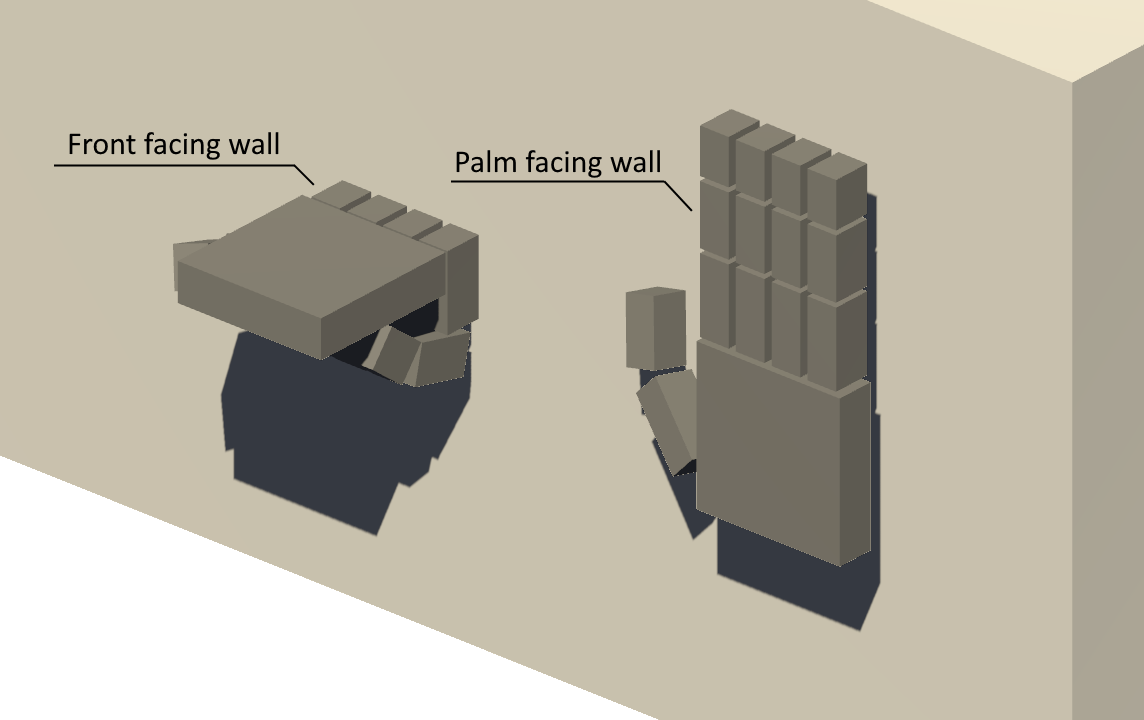
\includegraphics[height=6cm]{FacingDirection.png}
\caption{Diagram showing the two facing directions: The palm facing the surface and the front of the hand facing the surface.}
\label{fig:rotationHandFacingDirections}
\end{figure}

When rotation has occurred it's time to move the hand. In order for the hand not to penetrate the object it's moving towards, we sweep from the hand towards the controller position. When sweeping, we don't want the fingers to be taken into account. The accommodate for this, we don't have colliders on the fingers except for the fingertips. These colliders are disabled at all times, except during the calculation of the finger positions, which is described below. As mentioned before, Unity's $Rigidbody.SweepTest$ method doesn't detect objects that the hand is already touching, so we move it back slightly in the direction of the surface normal before sweeping. If the sweep hit an object the hand is moved to the hit position after which its slid across the surface to reduce the distance to the controller position. The sliding works in the same way as for the Sliding Rigid Hand (Section \ref{subsec:slidingRigidHand}). The normal is used to create a plane upon which the vector which spans between the hand position and the controller position is projected upon. This new vector is then what determines where to move the hand. If no object was hit during the sweep test, the hand is moved straight to the controller position.

The fingers of the Rotation Hand are moved using an inverse kinematics. When we want to move the fingers, there are two contexts we consider; either the hand is near objects that the fingers might interact with or it isn't. In both cases we start off by setting the fingers' targets to the positions defined by the controller's trigger value. This position is gathered from the hand animation, which is blended between an open and closed animation frame. In the case that there aren't any nearby objects nothing more is done to the fingers. When the player presses the trigger they will therefore close the hand and it will open, when they release the trigger. In the other case, where the hand is close to one or more objects, the fingers will be adjusted so that they don't penetrate any objects. To do this, all colliders within a radius are found using the same method described above. For each of the found colliders we check if the fingertips are inside by computing the penetration between the fingertip collider and the found collider. Before this step we enable the fingertip colliders, which are normally disabled. After computing the penetration we disable the fingertip collider again. The distance and direction gathered from computing the penetration is then used to move the finger's IK target. This means that the desired location the finger is trying to move to is moved outside of the object.

\begin{figure}[H]
\small
Position and rotation:
\begin{enumerate}[noitemsep]
\item If no objects are within a radius from the hand, move towards the position and the rotation of the controller and skip the rest.
\item Else find the orientation to rotate towards:
\begin{enumerate}[noitemsep]
\item Get the normal of the closest point on the closest object.
\item Get the current palm direction vector as the palm's up vector if the hand is open and the palm's negative forward vector if the hand is closed.
\item Calculate target direction vector by lerping between the current palm direction vector and the normal vector.
\item Calculate the rotation between the current palm direction vector and the target direction vector.
\item Rotate the hand towards the sum of the controller orientation and the rotation calculated in the previous step.
\end{enumerate}
\item And then move the hand:
\begin{enumerate}[noitemsep]
\item Move the hand a tiny bit in the direction of the normal (so the hand is not touching the object, when sweeping).
\item Sweep the hand towards the controller position.
\item If the sweep hit an object, place hand at hit point and slide to minimize the distance between the hand and the controller.
\end{enumerate}
\end{enumerate}
Finger positions:
\begin{enumerate}[noitemsep]
\item Set each finger's IK target to the animation's finger tip position.
\item Find all colliders within a radius from the hand.
\item If no colliders were found, skip the rest.
\item Else enable finger tip colliders.
\item Compute each finger tip collider's penetration with the colliders found in step 2.
\item Move each finger's IK target using the distance and direction found by computing the tip's penetration.
\item Disable the finger tip colliders again.
\end{enumerate}
\caption{Step-by-step process for placing the Rotation Hand and its fingers.}
\label{fig:stepByStepRotationHand}
\end{figure}

As mentioned, the Rotation Hand is the only of our prototypes that implement explicit rotation filtering, although it's a very simple version and only handles two cases. Both cases, the hand being open and the hand being closed, interact with all objects similarly. No matter the angle of approach, the size of the object or the type of object the Rotation Hand does the same thing. When open, it rotates so that when touching the surface the hand is placed flat on the surface with the palm first and when it's closed the front of the fist is placed against the surface. The rotation filtering works as intended for most surfaces, but could still be improved upon. One thing that feels a bit odd with the current implementation is that the hand also rotates to being palm front, when approaching objects with the back of the hand. Approaching an object with the back of the hand being closer than the front could be added as an additional case, where it might not rotate at all or perhaps rotates to let the hand be flat on the surface, but with the back of the hand against it instead of the palm. Other behaviors might also be preferable to the currently implemented cases for other object sizes and types.

While the rotation filtering works as expected in most cases, the fingers have some flaws that are quickly evident. The first problem with the fingers is due to the returning problem with depenetration; that it selects the closes point on the surface, which isn't always the best suited point. With the fingers the problem can arise, when the hand is placed such that the palm is touching the surface of a cube, but the fingers are pointing over the edge. When the fingers are bent to the point where they would be inside the cube the fingers would depenetrate to the same surface as the one the palm is touching resulting in an unnatural pose, which might also lead to the fingers to be placed partially inside the cube. The desired result would be that the fingers would be placed on the surface just around the edge from where the hand is, letting the fingers have a bend of around 90 degrees. As mentioned, the fingers can also end up being placed partially inside the cube, which is another problem. And this might even happen, even though the fingertips are placed on the correct surface in the cube example. This is the result of not depenetrating the hand as a whole. The hand is placed after which the fingers are adjusted, but only the tips of the fingers are depenetrated to find the location for the fingers' IK targets. The IK system doesn't take collisions into account, when moving the fingers to solve for the new target positions. This often results in the fingers partially penetrating the objects even after adjusting them, especially around edges and corners. As a final note, it's worth mentioning that this hand also uses a kinematic rigidbody, inheriting the same problems that comes with that as mentioned for the other prototypes above.

\section{Real Hand Visualization}
\label{sec:handVisualization}
When the hand is separated from the controller as happens with our prototypes when the controller is moved inside an object, it can be hard to understand exactly where one's real hand is positioned in the virtual world. Not knowing what the actual input to the hand is can lead the players to not understand why the hand is positioned as it is in the virtual world. To visualise the actual input to make it clearer to players what's happening, we've implemented a wireframe version of the hands, which is displayed at the position of the controller when the controller is separated more than a defined distance from the hand. The wireframe hand is placed such that it mimics where the virtual hand would have been placed, if it hadn't been obstructed, in essence showing where the players real hand is in the virtual world. As to not obstruct the players view too much by showing the wireframe hand immediately upon separation the distance is to fade in the wireframe, while the distance grows. This is implemented using one of Unity's animation curves as explained above, which fades the hand in by transitioning the alpha value from 0 towards 1\footnote{The alpha value indicates how transparent or opaque an object or image is. 0 means that it's completely transparent and 1 indicates that it's completely opaque.}. The result is that after the hand is separated from the controller by a certain distance the wireframe hand starts fading in and becomes more opaque when the distance increases further.

\begin{figure}[H]
\centering
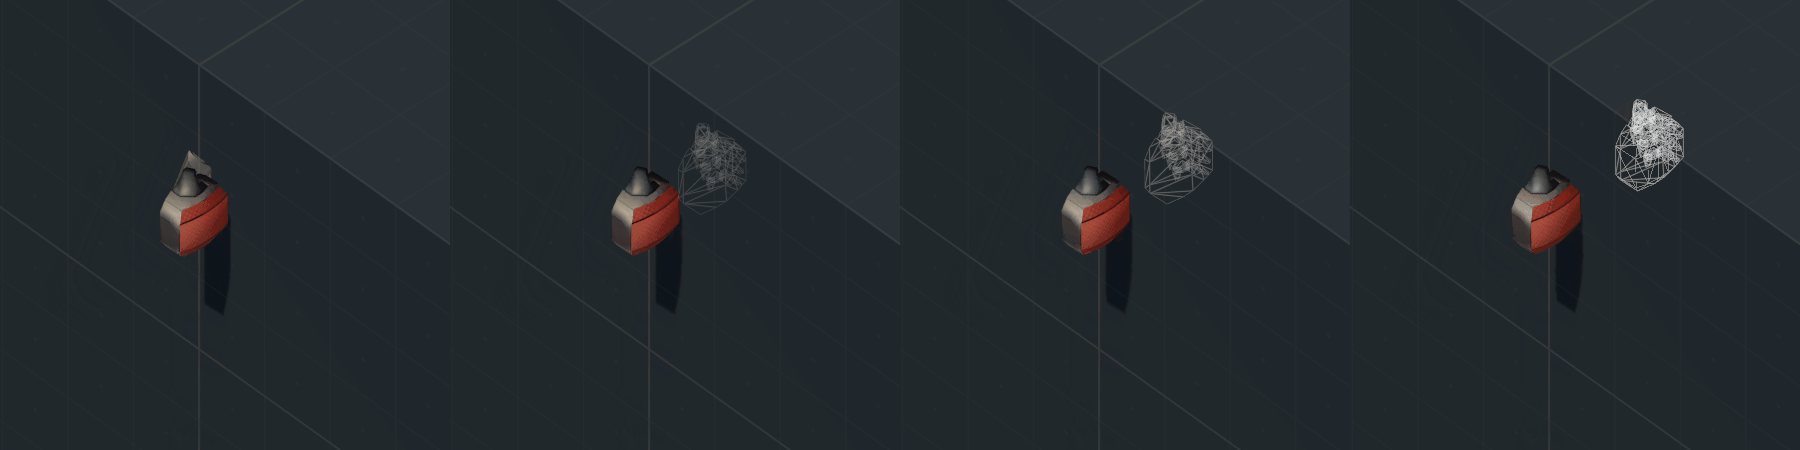
\includegraphics[width=\textwidth]{Sequences/Visualization/Seq_Visualization.png}
\caption{Sequence showing the real hand wireframe visualization. A gif can be found here: \url{https://tinyurl.com/HandVisualization} .}
\label{fig:visualization}
\end{figure}

\section{Haptic Feedback}
\label{sec:hapticFeedback}
Haptic feedback is about giving the user a sense of touch, when interacting with a system that otherwise doesn't allow for this. Examples of this can be buttons on touch screens, where haptic feedback can be applied to fill in the missing tactile feedback that is normally received from pressing a physical button. Haptic feedback works by applying forces, vibrations and motions to the user.

The HTC Vive controllers include hardware that makes haptic feedback possible. To access this feature from Unity we used the SteamVR plugin by Valve, which can be found on the Unity asset store. SteamVR functions as a wrapper for the HTC Vive and makes setup and use it easier\footnote{SteamVR can also be used for other Headsets like the Oculus Rift.}. SteamVR allows a pulse to be triggered on the controller with a pulse length in microseconds as the parameter. The length here is not used to make the vibration take more time, but is to make it feel stronger. Features like vibration duration and pulsed vibrations (vibrations with gaps) is up to the developers to implement. We implemented an intermediate layer to allow us to do these with a single method call as the interface called Rumble. This method allows us to start a vibration for a controller with a given duration, intensity and interval. The duration is the duration of the vibration in seconds, the intensity is the pulse length described above and the interval is the gap in seconds between pulses. For each vibration, these values can be set differently giving a different kind of feel. Setting these values, however, isn't as trivial as it might sound. Especially the intensity and the interval has a lot to say in how the vibration feels to the player and they affect each other, meaning that changing the intensity might require the interval to be changed to make the vibration feel right again.

Our main use of haptic feedback is when interacting with objects in the virtual world, for instance when hitting an object with a hand. To streamline the process of adding haptic feedback to objects in the world, we created the Rumbler component. The Rumbler component can enable haptic feedback in four different scenarios: When the object is hit by the hand, when the hand slides over the surface of the object, when a joint attached to the object breaks while it's grabbed by the hand and when the object is dropped by the hand. Each of these features can be enabled or disabled for the object individually and have their own settings for determining strength and duration of the vibrations. The first three of these use Unity's animation curves to define the intensity of the vibration. When hitting objects the animation curve's input is the magnitude of the impulse resulting from the collision. When sliding over objects, the input for the animation curve is calculated using the velocity of the hand then multiplying it with the average friction values from the hand's and the object's physics materials\footnote{Unity uses physics materials to store values such as dynamic and static friction and bounciness and other settings used by the physics system. Physics materials are applied to colliders.}. For the joint break, the evaluation value is the break force, which is the force applied to the joint, which caused it to break. These are all normalised before being used with the animation curve by dividing them with a set max value and then clamping the result to be between 0 and 1.

When interacting with objects that have the Rumbler component attached the settings set for the Rumbler's four interaction types dictates the vibration caused in the controller. When hitting a wall, for instance, the wall's attached Rumbler's settings for hitting dictate, what values to use for the duration, intensity and interval, when calling the Rumble method described above. In the case of hitting the intensity is calculated based on the animation curve set up for the Rumbler component and the magnitude of the impulse of the collision.


% NOTE: Difference between rumble and haptic feedback: https://www.reddit.com/r/oculus/comments/56ocxy/whats_the_difference_between_rumble_and_haptics/

% NOTE: Haptic feedback for the Vive controller: https://steamcommunity.com/app/358720/discussions/0/405693392914144440/

\section{The Grabbing System}
\label{sec:grabbingSystem}
The grabbing system is first and foremost about grabbables. Grabbables (or grabbable objects) are objects that can be grabbed with the hand, when the trigger is pressed passed a certain threshold. In our implementation it's the same as for when the hand is closed. We've implemented three different grabbable variants, which all have the same goal, but have different approaches and thus different pros and cons: The Parenting grabbable, the Fixed joint grabbable and the Velocities grababble. When a grabbable object has been grabbed it follows the hand as long as the trigger is held pressed. The grabbable can then be dropped or thrown by releasing the trigger again. The Fixed joint grabbable and the Velocities grabbable can also be dropped, if a large enough force is applied to the grabbed object, which can occur if the grabbed object hits something, for instance. Grabbable objects also all have a rigidbody component attached to them so they interact with the physics system and finally, as mentioned above, the Physics Hand uses the fact that it's hovering over a grabbable to indicate that the object can be grabbed by filtering on the finger positions.

The Parenting grabbable does what the name indicates. It makes the hand the parent object of the grabbable object when grabbed. When a parent object is moved or rotated its children are moved and rotated as well. This makes parenting one of the easiest ways of making one object move another, but it also has its downsides. The Unity documentation states that when an object is under physics control, which objects with a non-kinematic rigidbody are, they move semi-independently of the way its transform parents move \parencite{UnityManualRigidbody2017}. This is an issue, because the grabbable objects all have non-kinematic rigidbodies attached. If nothing is done about this, there could be problems with the collisions and other calculations when the parents are moved and objects would still fall due to gravity. Furthermore, sweeping with the parent rigidbody wouldn't include the colliders of the child rigidbody as well, resulting in wrong placements of hands while grabbing objects. Since rigidbodies can't be disabled directly, we solved this problem by saving all the rigidbody values, removing the component and then when the grabbable object was released, we added back a new rigidbody component and reinstated the saved values. Furthermore, throwing of objects needs to be implemented manually, when using the Parenting grabbable, because the moment it's moved back outside of parenting and it's received its new rigidbody component, it will just apply gravitation and fall straight down or perhaps get pushed a bit by interacting with the hand after release. To implement throwing we save a history of the velocity and angular velocity of the controller over a certain number of frames. The averages of these velocities are then applied to the grabbable's rigidbody after separating it from the hand. This results in a direction and velocity for the grabbable that feels satisfactory. Using the grabbed object to push other objects, however, have certain problems which are tied to the use of kinematic rigidbodies (which of course doesn't apply to the Physics Hand). When the grabbable is a child of an object with a rigidbody, it becomes part of that rigidbody. So while an object is grabbed, it's part of the hand's rigidbody. One of these problems occurs when trying to push a dynamic object into an immovable object, in this case using a grabbed object to do so. The object being pushed will be locked between two bodies that aren't affected by the physics system, so the object in the middle can't push the object on either side away, resulting in the squeezed object being unstable and jumpy.

The Fixed joint grabbable is implemented using one of Unity's fixed joints. A joint is used to attach a rigidbody to another or to a fixed point in space. Different joint types exist that have different behaviors. The Fixed joint grabbable, as the name states, uses a fixed joint to lock the grabbable to the hand, when grabbed. By using a fixed joint, the grabbable has forces applied to it, which makes it move to the position and rotation indicated by the joint. This target position and rotation is defined when the joint is created and is set as the position and orientation the grabbable object has relative to the hand at that time. One problem that occurs, if the hand stops abruptly after moving fast, is that the grabbed objects has a bit of a spring effect, first overshooting the target and then bouncing back. This problem is what the Velocities grabbable tries to solve. Another effect of using a joint is that the grabbable can be pushed away from its target location, by forcing it into other objects, which can lead to situations, where the hand is suddenly not facing the grabbed object from the same direction as before or the hand is in an unrealistic position to be able to hold the object.  Joints also have options that enable special effects like the breaking of the joint, when an applied force (or torque) is larger than a certain threshold. We make use of this to allow the behavior of dropping grabbed objects when hitting them into immovable objects, for instance. When an object has been grabbed and the object is smashed into a wall, depending on the object, dropping it can add a feeling of realism. In our implementation each object can define their own break forces so they can be customised to fit with their use and expected behavior.

The Velocities grabbable is moved along with the hand in the same way the Physics Hand is moved. When grabbed, the current position and orientation relative to the hand is saved as the target and when the hand moves, so does the target. Then every frame the velocity and angular velocity needed to reach the target position and rotation is calculated and applied to the object. The gravity doesn't need to be disabled for the grabbable's rigidbody, since we overwrite the velocities each frame. Setting the velocities of the grabbable instead of letting the joint apply forces, removes the springiness seen with the Fixed joint grabbable, when suddenly stopping after having moved fast. The issue with the object being able to be separated from its target position and orientation still persists, though. As an addition to the Velocities grabbable, compared to the Parenting grabbable, we wanted to implement the effect of dropping the object, when hitting it hard into other objects. This was given to us by using joints for the Fixed joint grabbable. To implement it here, we decided to go for a max separation in distance and rotation from the target as the threshold for when to drop the grabbed object. When either the distance between the grabbbable and its target was too large or its rotation was to far off, the object would be dropped from the hand, simulating the effect of breaking the joint for the Fixed joint grabbable. The implementation of the Velocities grabbable makes it look and feel very much like the Fixed joint grabbable, just without the springiness problem described.

As a final note about the grabbing of objects, it's worth noting that the Physics Hand also allows for lifting objects without grabbing them using the trigger in a stable manner. As mentioned above, lifting has benefits like giving a sense of weight to objects and disallowing objects that are too heavy to be carried. Even if an object is too heavy to carry, it might still be light enough for it to be pushed or rolled. This gives a completely different feel to the act of carrying objects than grabbing with the trigger, although using the trigger method gives a very high amount of control over the grabbed object, as lifting requires the player to look at the object to be able to see how their hands are interacting with the object, while grabbing it with the trigger locks the object to the hand and the player doesn't need to think about dropping it except for when the grabbed object hits another object hard enough and it's dropped.

\section{The Baseline: Our Job Simulation Hand}
To be able to evaluate our prototypes, we decided to implement a version of the hands as they feel in the game Job Simulator, mentioned previously. The main focus points of the Job Simulator Hand and the examples that we've already mentioned above are the fact that it isn't constrained by immovable objects in the virtual world and will freely penetrate objects and when it is used to grab objects the hand becomes hidden. We've implemented a hand which we've tried to get as close to the hands from Job Simulator as possible and in this section we'll go into details about the implementation of this hand in the same way as we've described the prototypes above.

In our implementation of the Job Simulator Hand, it is set up using a kinematic rigidbody, which has its flaws and benefits as described above. The hand is moved by using Unity's $Rigidbody.MovePosition$ and $Rigidbody.MoveRotation$, which we also used before for some of the prototypes. It has no position filtering to stop it from penetrating objects, so it will always keep the position and orientation of the controller it's following. As in Job Simulator, our implementation also indicates, when the hand is near objects that can be grabbed, by bending all the fingers slightly. As with the Physics Hand, we detect, when there is a grabbable inside its grab area upon which we bend the fingers. Unlike the Physics Hand, though, we just use a set hover closed value as the closed value of the hand, when hovering over a grabbable. So when the grab area is empty, we use the player's input for the closed value of the hand and set the animation to blend accordingly. When there is a grabbable object in the grab area, we overwrite the input with the defined hover closed value. When the new closed value has been defined, we lerp towards it to smoothen out the motion of the fingers. One thing that none of our prototypes do, but the implementation of the Job Simulator Hand does is to hide itself, when grabbing objects. When an object has been grabbed by closing the hand while hovering over a grabbable, we disable all renderers\footnote{In Unity a renderer is a component, which renders a mesh, making it visible in the world.} for the hand, effectively making it invisible. When the object is released or dropped the renderers are enabled again.

\begin{figure}[H]
\centering
\small
Position and rotation:
\begin{enumerate}[noitemsep]
\item Move the hand's rigidbody to the target controller using $MovePosition$.
\item Orient the hand's rigidbody compared to the target controller using $MoveRotation$.
\end{enumerate}
Fingers:
\begin{enumerate}[noitemsep]
\item Check if there is a grabbable object in the grab area of the hand below the palm.
\item If there is, set the new target closed value to a defined hover closed value.
\item If there is not, set the new target closed value to the trigger input value.
\item Lerp towards the new target closed value and update the hand animation accordingly.
\end{enumerate}
\caption{Step-by-step process for placing the Job Simulator Hand and its fingers.}
\label{fig:stepByStepJobSimHand}
\end{figure}

\section{Chapter conclusion}
\label{sec:CHAPTERCONCLUSION}

\todo[inline]{Find better section name}

In this chapter we've delved into the categorization of approaches, which describes what position filtering, rotation filtering and filter position filtering is, how they can be implemented on a high level and how they've been used in our prototypes. Our use of these filters has had the goal of making the hands behave in a more realistic way than the what is seen in games like Job Simulator. We've used position filtering as the main driving force behind stopping penetration of objects and we've used rotation and finger position filtering as a means to let the hand get closer to the target controller, while adhering to the restriction of not penetrating objects. Furthermore, the finger filtering has also been used as a diegetic way of displaying to the player which objects are grabbable and which aren't.
The grabbable system we've implemented has the goal of making it easier to setup which objects can be grabbed by the hands and which can't. The grabbables come in three variants, the Parenting grabbable, the Fixed joint grabbable and the Velocities grabbable. The Parenting grabbable was the first implementation we made and might be the naïve solution. The grabbed object set to be a child of the hand, meaning that when the hand's transform is changed, so does all the children, including the grabbed object. The Parenting grabbable comes with its own set of troubles due to having two rigidbodies, one being a child of the other. This can create situations with the physics system and therefore needs to be handled. Our solution was to remove the grabbed object's rigidbody and replace it again after the object has been dropped. A more elegant solution though could be to not make the object a child of the hand, but to somehow connect it to the hand by other means. One of these solutions is to use a joint to connect the two rigidbodies; the grabbed object's and the hand's. The Fixed joint grabbable uses a fixed joint, which always tries to move the rigidbody to its target location by applying forces to the object. Moving this way means that the hand and the grabbed object will interact as separate bodies with the surrounding environment, but the fact that the movement happens through forces creates this bouncing effect, where the grabbed object overshoots its target and bounces back and forth. As a means to solve this problem, we experimented with setting the velocities of the Grabbed object in the same manner we do when moving the Physics Hand to its target position. The velocities needed for the object to reach its target in one frame are applied to the object and by moving it this way, we see the same kind of behavior as with the fixed joint, but without the bounciness seen when moving the controller fast and then stopping suddenly.

To further improve upon the feel of the hands, we implemented the visualization of the player's "real hand", which displays the where the hand would have been without the any filtering. This helps the user understand where the filters originate from and what their actual input is, even though the virtual hand is constrained by the world around it. But to indicate when players were touching objects with the virtual hand and to indicate other types of interactions, haptic feedback was put in place. The haptic feedback works by vibrating the controllers with certain intensities and intervals over a duration. This vibration can be used to signal to the player that they were stroking or hitting objects or to indicate when events like the dropping of objects occurred.

The hand prototypes along with these additional systems try to solve certain problems. These problems include enforcing physical constraints on the hand, for instance that it shouldn't be able to penetrate objects. Furthermore using visualization and finger filtering, the prototypes try to reduce confusion and increase understanding of the systems, by letting the players know, when they crossed boundaries and are near interactive objects. There are problems, though, that none of the prototypes solve. One problem that all of the prototypes have in common is introduced, when the hand is constrained by an object, where the controller is inside it. When moving the controller sideways, the hand slides over the surface, but when the hand reaches an edge and the controller is now outside the object, but far away from the hand the hand jumps or lerps to the position of the controller. This movement, where the hand tries to correct for the distance between itself and the controller feels unnatural, but also emanates from a situation that can't exist in the real world. Another issue, which is related to the use of kinematic rigidbodies is the fact that they don't play well forcing other non-kinematic objects into each other or into immovable objects. These issues have already been described above, but our solution so far has been to use the Physics Hand, which has fewer of these issues due to that it can be affected by its surroundings and allows the physics system to handle such conflict.

For these reasons our preferred setup amongst our prototypes and systems is the combination of the Physics Hand and the Velocities grabbable using real hand visualization and haptic feedback, which has the least amount of unhandled cases that we've found and is therefore also the prototype we chose to use during our user evaluations.